\chapter{Verification and testing}

\section{Testbench}



\begin{code}
    \inputminted{vhdl}{listings/04/CORDIC_tb.vhd}
    \captionof{listing}{\texttt{CORDIC\_tb.vhd}}
    \label{code:testbench}
\end{code}


\section{Error verification}

\cadm{ho fatto su circonferenza di 31 non so perchè, devo fare su circ di 127}

The implementation of the CORDIC algorithm in vectoring mode for Cartesian-to-polar conversion demonstrates 
exceptional accuracy in both the module (\( \rho \)) and phase (\( \theta \)) outputs. Using a fixed-point 
representation of \( Q8.8 \) for \( \rho \) and \( Q3.13 \) for \( \theta \), the errors were summarized as follows:

\[
\text{Module Error:} \quad \text{Max} = 0.003938 \, \text{units}, \quad \text{Mean} = 0.001889 \, \text{units}
\]
\[
\text{Phase Error:} \quad \text{Max} = 0.000153 \, \text{rad}, \quad \text{Mean} = 0.000061 \, \text{rad}
\]

The test was performed on 512 × 512 input points uniformly distributed within a circle of radius 127. 
This range ensures a comprehensive evaluation of the algorithm over a high range of valid input values while maintaining 
consistency with the precision of the fixed-point formats used. The fixed-point representation employed provides a precision 
of \( 2^{-8} \) for \( Q8.8 \) (module) and \( 2^{-13} \) for \( Q3.13 \) (phase). 
\\\\
The observed errors are well within these precision limits, with all measured deltas smaller than the respective numerical precision of the formats. Any discrepancies between the input and output values are solely due to the conversion of these fixed-point representations into real numbers for plotting and analysis. 
\\\\
The 3D plots of module and phase errors visually confirm the bounded and negligible nature of the errors across 
all tested input combinations. Assuming no error on the input, this analysis validates that the algorithm introduces 
no significant error in the output, demonstrating the precision and robustness of CORDIC algorithm implementation with 24 bits internal logic.

\begin{figure}[h!]
    \centering
    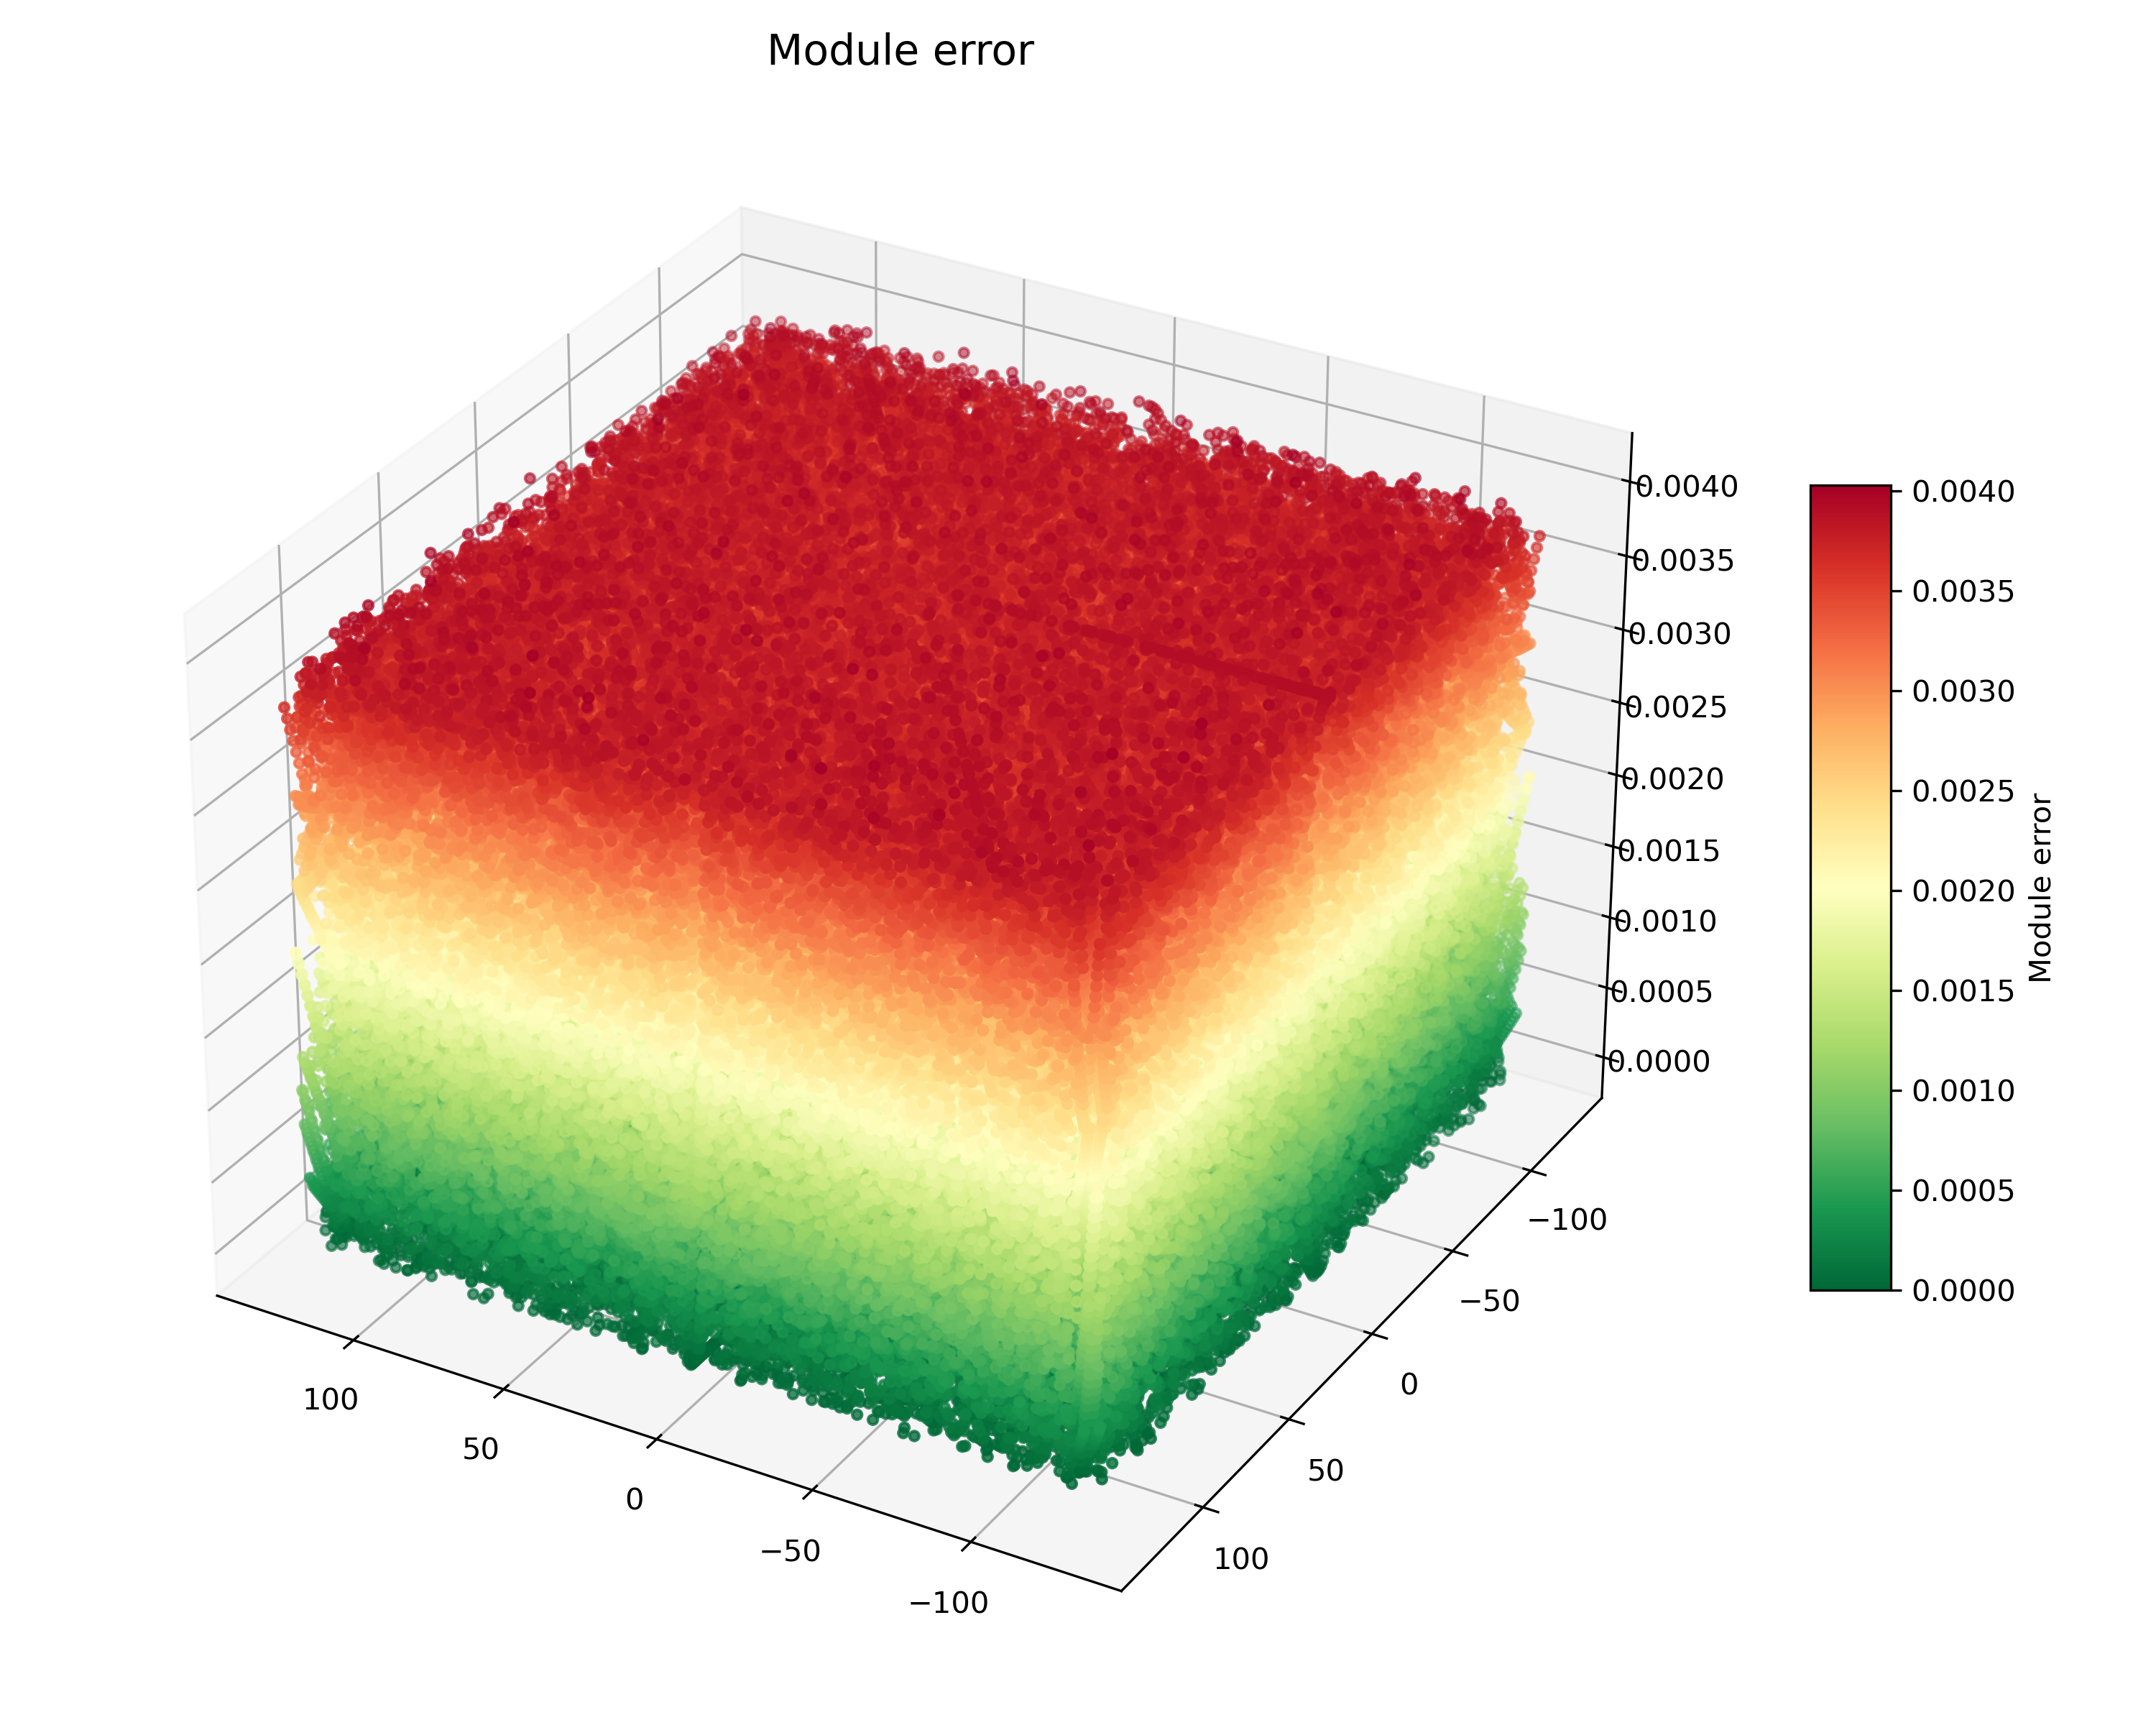
\includegraphics[width=0.8\textwidth]{./images/Verification/module_error.png}
    \caption{3D plot of module error (\( \rho \)).}
    \label{fig:module_error}
\end{figure}

\begin{figure}[h!]
    \centering
    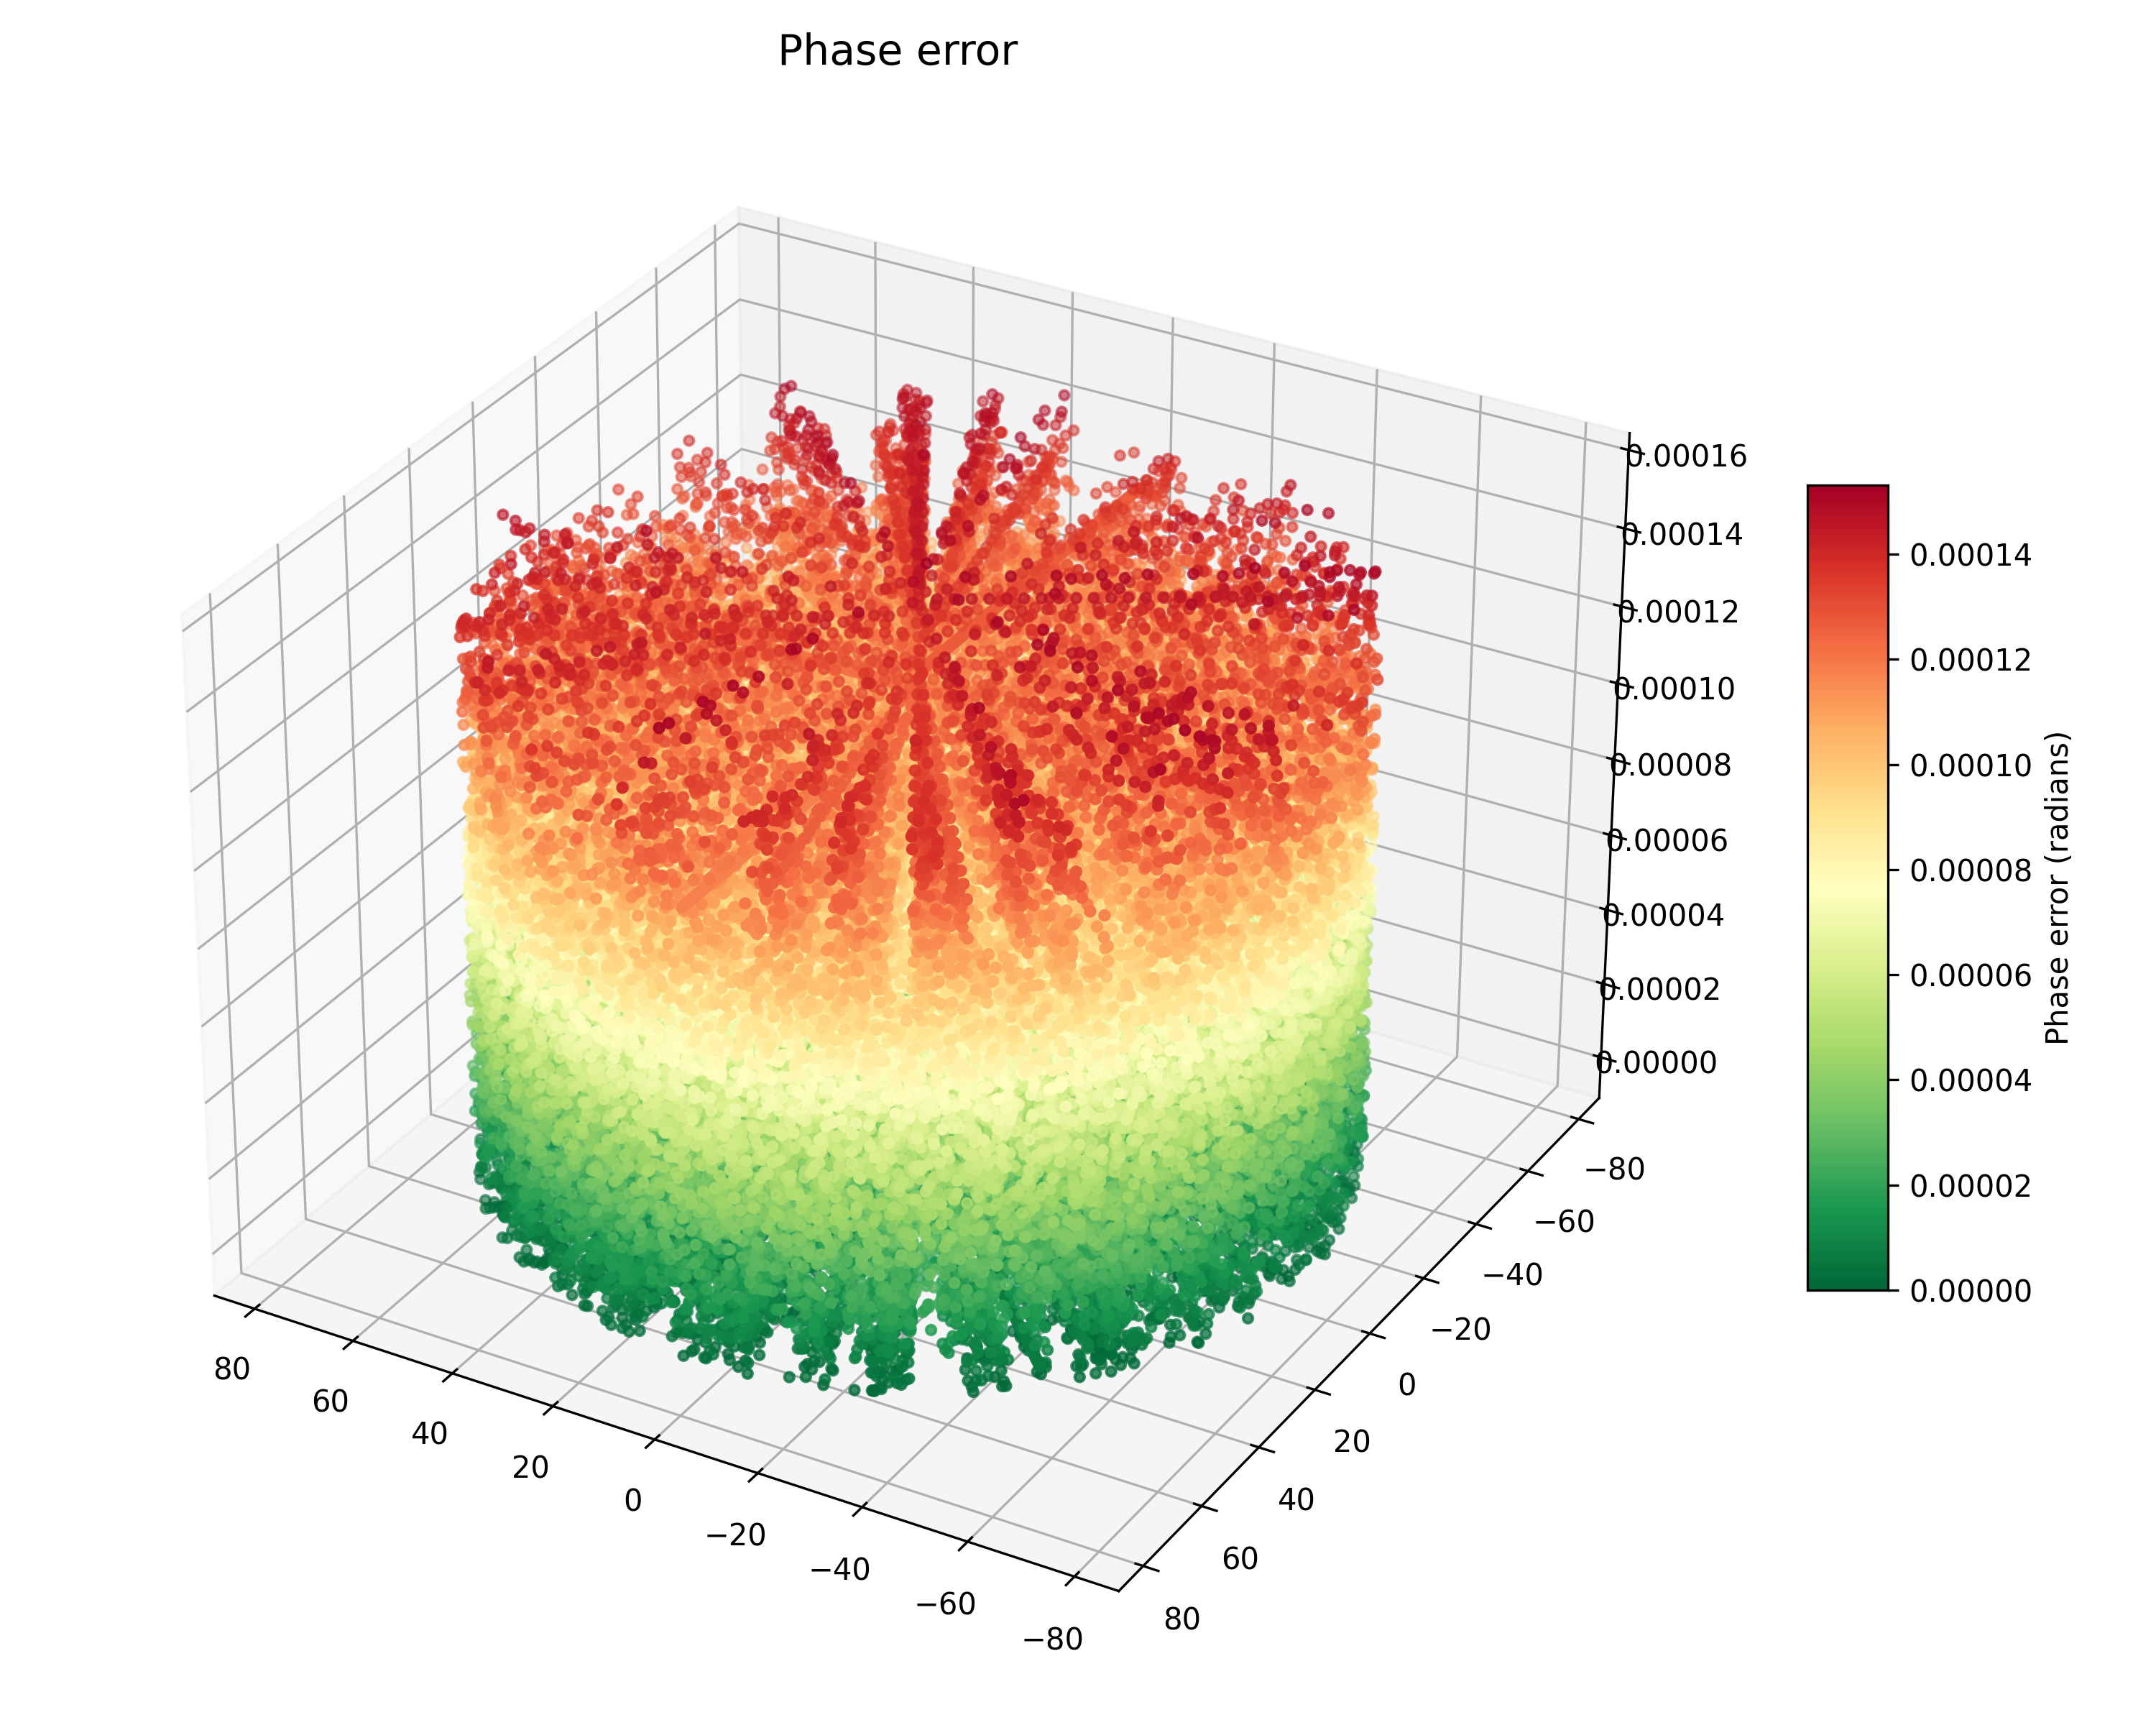
\includegraphics[width=0.8\textwidth]{./images/Verification/phase_error.png}
    \caption{3D plot of phase error (\( \theta \)).}
    \label{fig:phase_error}
\end{figure}
